% !TEX root = ../00_thesis.tex

%-------------------------------------------------------------------------------
\section{Implementating \DRP}
\label{sec:drp_implementation}
%-------------------------------------------------------------------------------

This dissertation aims to provide concrete solutions for wireless \CPS, not only theoretical concepts. It is therefore important to implement the concepts and evaluate their performance when running on real hardware.
This section presents some important design choices we made for our implementation of \DRP.
%
The performance evaluation is presented in \cref{sec:drp_evaluation}.

%-------------------------------------------------------------------------------
% \subsection{Design Choices}



\DRP extends \blink~\cite{zimmerling2017Blink}, which is a real-time scheduler for LWB~\cite{ferrari2012LWB}. Thus, we start our implementation of \DRP from an existing implementation of LWB~\cite{Code_LWB}. There are two main functionality to implement for running \DRP:
\begin{itemize}
  \item
% (i)~
compute \blink schedules, and
  \item
% (ii)~
perform \DRP admission tests.
\end{itemize}

\DRP leverages the \DPP design by having all the computations performed by the \AP while the \CP only runs LWB.
From an implementation stand-point, the challenge is that the \AP does computations but the \CP needs the results (\eg the LWB schedules); the communication over \bolt between \AP and \CP  must happen in a way that does not interrupt or delay LWB operations.
Moreover, the memory and computational requirements of the protocol must be compatible with the (typically limited) capacity of embedded hardware.

\fakepar{Task distribution}
On all nodes, the computations related to \DRP admission tests are performed by the \AP, including \CP's buffer checks~(\cref{thm:CP}).
These tests only require minimal state keeping, which can be easily delegated to the \AP. This has two benefits: (i)~it limits the modification to the \CP firmware (\ie LWB) and (ii)~it improves performance (the admission test is more efficiently computed by the \AP than by the \CP).

\fakepar{Round structure}
Our implementation maintains the original LWB round structure, only removing the contention slot~(\cref{fig:drp_round}). This slot becomes redundant in \DRP since each node bootstraps with registered control flows, which are used for further \DRP requests and flow registrations~(\cref{sec:designDetailed}).

\begin{figure}
  \centering
  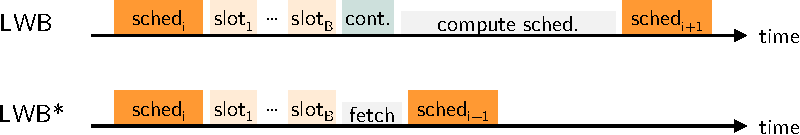
\includegraphics[scale=1]{drp_round}
  \caption{The original LWB (Top) and the modified round used in \DRP (Bottom).
  \capt{\DRP removes the contention slots, made redundant by the presence of dedicated control flows. Furthermore, the time span before sending the next round's schedule can be significantly reduced: indeed in \DRP, the host \CP can quickly fetch the schedule from the \AP, which has done the computation in parallel.}}
  \label{fig:drp_round}
\end{figure}

\fakepar{Schedule fetch}
The host \CP fetches the schedule for the LWB round $i+1$ at the end of round $i$~(\cref{fig:drp_round}).
\CP requests the schedule to \AP, which maintains the schedule ready and writes it to \bolt whenever the request comes.

\fakepar{Communication model}
The communication between \AP and \CP over \bolt can be based on polling or interrupts. When using polling, processors asynchronously check the status of their incoming \bolt queue to check whether a message is present. Conversely, an interrupt can be generated at the receiving processor whenever a \bolt \texttt{write} operation is completed.
\begin{description}

  % \item[\AP $\boldsymbol{\rightarrow}$ \CP]
  \item[\AP to \CP]
  When \AP writes to \bolt, we trigger an interrupt on the \CP and read out the message immediately.
  Since \DRP flow model is sporadic and new packets are expected infrequently~(\cref{sec:problem}), using interrupt is fast, energy efficient, and avoids building up the \bolt queue.

  However, during LWB rounds, it is paramount that \CP operations are not delayed or disturbed. Thus, during the rounds, interrupts are disabled and (potential) new messages written by \AP are read out after the round.

  % \item[\CP $\boldsymbol{\rightarrow}$ \AP]
  \item[\CP to \AP]
  We assume that the \AP on the host node is dedicated to its role of host (\ie there are no other application tasks running of that \AP).
  Thus, we use interrupts, which allows for fast reaction times from \AP to \CP's requests (\eg when fetching the next round's schedule).
  When \CP receives a \DRP request, the \AP immediately reads out the request, stores it in a request queue~(\cref{fig:AP_alternatingbuffer}), then processes incoming requests whenever possible~(\cref{fig:AP_statemachine})

  For the other nodes, the decision of using polling- or interrupt-based communication depends on the timing requirements of the application.
  Our implementation supports both modes.
  For simplicity, we use interrupts in our evaluation~(\cref{sec:drp_evaluation}).

\end{description}

\fakepar{Host \AP state-machine}
The host \AP is responsible to compute the \blink schedules and to perform the admission tests for incoming \DRP requests. As processing \DRP requests takes a variable (and possibly long) time, priority is given to the schedule computation: as soon as the schedule for the round $i$ has been fetched by the \CP, \AP computes the schedule of round $i+1$.

Once the schedule is ready, \AP continues with the processing of \DRP requests. After each processed request, if the flow is admitted, \AP recomputes a schedule for round $i+1$ taking the new flow into account. The procedure repeats until the schedule is fetched by \CP or when all requests have been processed. The host \AP state-machine is illustrated in \cref{fig:AP_statemachine}.

\afterpage{
\begin{figure}
 \centering
 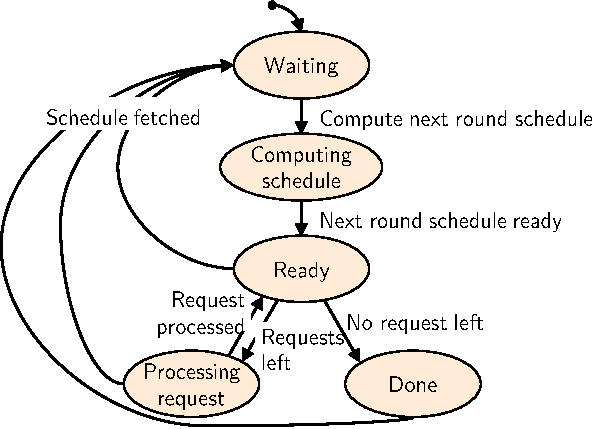
\includegraphics[scale=1]{AP_statemachine}
 \caption{State-machine of the host \AP.
 \capt{
  \AP first computes a valid schedule for the next round. Then, the \AP processes queued \DRP requests, one at a time, and recomputes a (new) schedule accounting for the newly admitted flow.
 }}
 \label{fig:AP_statemachine}
\end{figure}

\begin{figure}
 \centering
 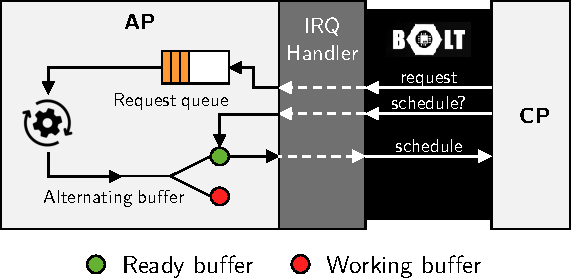
\includegraphics[scale=1]{AP_alternatingbuffer}
 \caption{Request queue and alternating buffer on the host \AP.
 \capt{
  Incoming messages from \CP trigger an interrupt and are handled immediately.
  \DRP requests are put in a dedicated queue for later processing~(\cref{fig:AP_statemachine}).
  When \CP writes a schedule request, the interrupt handler fetches the most recent schedule from the ``Ready buffer'' and write it to \bolt.
 }}
 \label{fig:AP_alternatingbuffer}
\end{figure}
}

\fakepar{Alternating buffers}
As described above, the host \CP fetches the next round schedule from its \AP, which sends a valid schedule immediately.
However, this conflicts with the admission of new flow requests: the \AP may be processing a request (including the computation of a new schedule) when \CP requests the schedule.

We handle this situation using an alternating buffer for the next round schedule~(\cref{fig:AP_alternatingbuffer}). One buffer is used to store a valid schedule for the next round, which the \AP computes first. After each \DRP request is processed, the newly computed schedule is written into the other buffer. The process repeats until all requests are processed.

Hence, even if \CP fetches while \AP is writing a schedule in one buffer, the other buffer still contains a valid schedule, which can be immediately sent to \CP over \bolt.
This guarantees a fast transmission of the schedule from \AP to \CP while avoiding memory corruption on the \AP.

\begin{remark}
  Alternative design choices and their respective benefits are further discussed in Andreas Biri's Master Thesis~\cite{biri2017Unleashing}.
\end{remark}
